
\documentclass[12pt]{article}
%	options include 12pt or 11pt or 10pt
%	classes include article, report, book, letter, thesis
\usepackage{graphicx}

\author{Adam Blance 40161070}
\date{29 February 2004}

\begin{document}

	\title{SET10108 Concurrent and Parallel Systems \linebreak Coursework 2 \linebreak N-Body Simulation}
	
	\markboth{40161070}{}
	\maketitle
\begin{abstract}
			
\end{abstract}
	
\section{Introduction}
As more and more of our world becomes heavily reliant on data found online, it becomes incredibly important to learn how to parallelise this data to allow data to be processed as quickly as possible.  Learning how to parallelise sequential systems has become a very important skill to possess in your repertoire. 
\newline 
In this coursework the task was too parallelise a ray tracer to improve the performance using multi-threading and CPU- level parallelism. Then evaluate the performance and compare it to the serial performance.  The ways that the algorithm was evaluated was through changing several aspects such as samples per pixel and size of image. These aspects were then measured through speed up and efficiency and recorded.
\newline
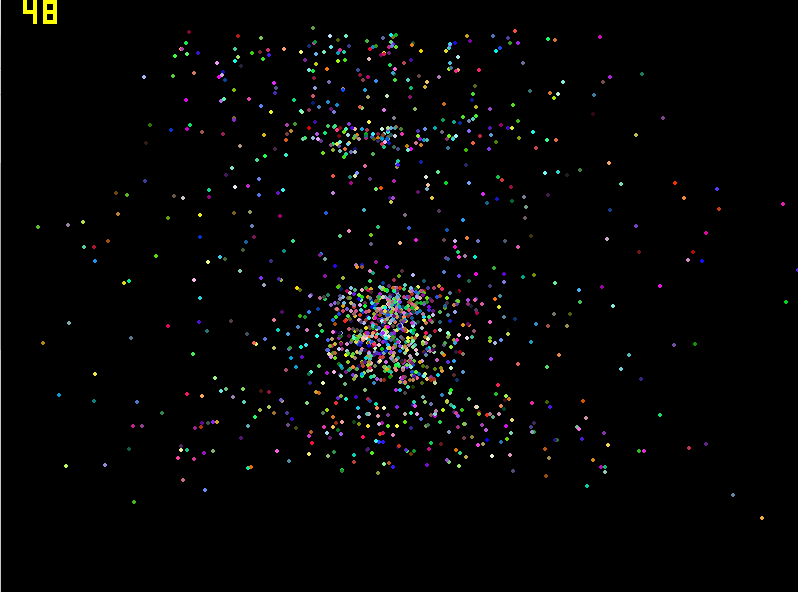
\includegraphics[scale=0.5]{pics/intro.png}

\section{Inital Analysis}
The first task in the course work was choosing which of the three tasks posed to us. It was decided that N-Body simulation would be the task that would be selected. The reason for deciding on N-Body simulation was because research into JPEG compression found little results and while prime numbers search was possible, N-body was chosen down to personal preference.
\newline 
Once this was decided on research was conducted into N-Body simulation and which algorithm online would be used to parallelise. During the search many possible candidates were found but the best one was harrism/mini-nbody . The reason for this was it because of its relative simplicity allowing for graphical output to be easily added into the code. After that small tweaks were made to the N-Body simulation and using Allegro 5, a graphical interface was created. From this point the inital anlysis was conducted.
\subsection{First Results}
It was decided that 3 things would be tested to gather the baseline data of the application to discover any bottlenecks. These were:
\begin{itemize}
 \item Length of Simulation.
 \item Size of Times Step.
  \item Number of Particles. 
\end{itemize}
These three factors were measured by the execution time, this was calculated by taking using the system clock and printed to a console, also taken was the average framerate this was measured using Fraps. The tables for the measurements are shown below.
\subsubsection{Length of Simulation}
\newline
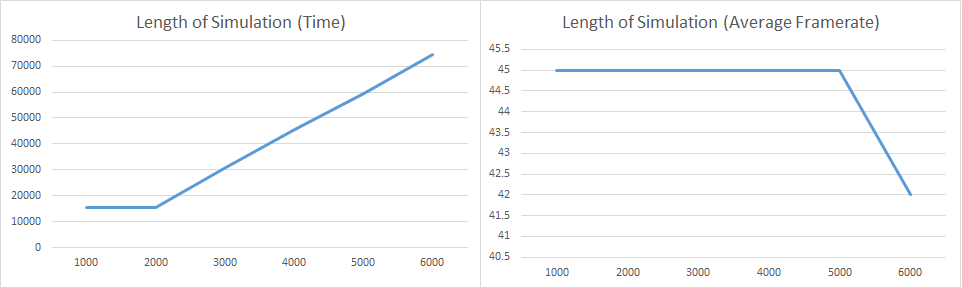
\includegraphics[scale=0.5]{pics/ialength.png}
\newline
The reason for measuring the length of the simulation was to see if a drop off occurred at any point and performance suffered because of this. This was measured in number of iterations. As shown in the results no bottleneck occurred at any point as the time taken increased at steady amount as was expected and the framerate did not suffer at all. An anomaly occurred during this test. This being the framerate dropping to 42 fps rather the holding at 45 fps like the other tests this probably had nothing to do with code and with assumed to be an anomaly. The other strange occurrence in this test was that ///comeback to this /////
\subsubsection{Size of Times Step}
\newline
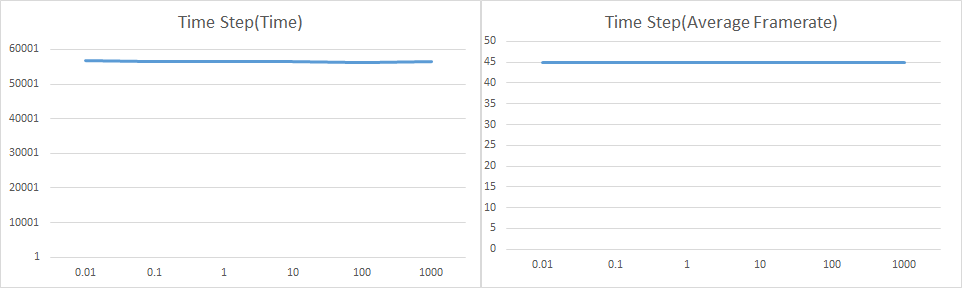
\includegraphics[scale=0.5]{pics/iatime.png}
\newline
The size of times step is how long between the measurements are taken in the application. This was measure as with a higher time step, the quicker the particles move on the screen. This could cause a bottleneck to occur with more happing on screen the framerate could drop, however as shown in the graph the framerate remained constant, as did the time taken when the time step was increased.
\subsubsection{ Number of Particles}
\newline
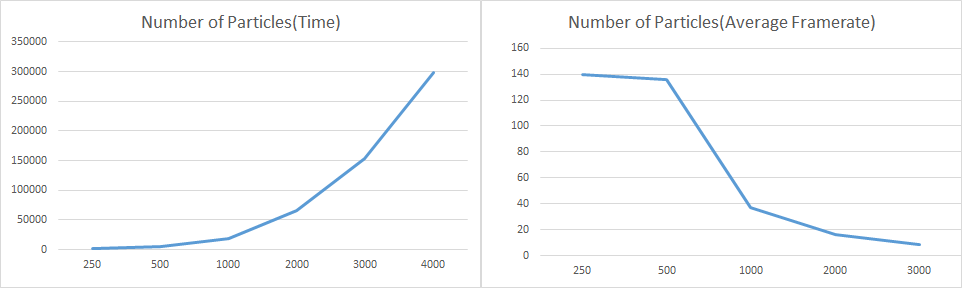
\includegraphics[scale=0.5]{pics/ianumber.png}
\newline
The final measurement that was taken was Number of Particles the graph show clearly that a bottleneck occurs as the number of particles increases. This is what will be tested once the code is parallelized. 
	
\section{Methodology}
To test the parallelisation of the ray cast algorithm three aspects of the code were tested; the number of samples per pixel, changing the size of the image and adding other objects to the scene. To keep the results consistent only one value was tested at a time. The other values were kept constant while the tests were being run. The time taken to complete the image was measured, this was repeated 10 time and an average was calculated. These test were time consuming so other computers were used however all the computers used had same graphics card and CPU to allow the tests to stay legitimate. 
	\subsubsection{OpenMP}
	The first approach was to use OpenMP, OpenMP is a library to support shared memory concurrency allowing it to be portable and added easily to the program. The reason OpenMP was used over the first for loop as the first approach was because it’s simple to use which means it will also be rather robust as it will help the programmer tag parts of potential concurrency. It can also be used in conjunction with other approaches allowing more threading to be used.
	\subsubsection{CUDA}

	
	\section{Results}
	\subsection{Discussion}
	
	\section{Conclusion}
	

	
\end{document}